\chapter{Estado de la Cuestión}
\label{cap:estadoDeLaCuestion}

El objetivo de este capítulo es analizar el panorama actual de las herramientas de apoyo al aprendizaje de la programación y los sistemas de evaluación automática. Para el correcto desarrollo de este proyecto, es necesario comprender las tecnologías existentes e identificar carencias en la interacción entre el sistema y el usuario.
A continuación, se presenta un análisis comparativo de diversas plataformas que permitirá contextualizar nuestra propuesta.

\section{Acepta el reto}
https://aceptaelreto.com/ es una de las plataformas de programación competitiva más utilizadas, se centra en la resolución de problemas algorítmicos con un enfoque de competición. Su relevancia para este proyecto reside en su modelo de gestión y categorización de problemas algorítmicos. Destaca por su robusto sistema de envío y evaluación en tiempo real, proporcionando al usuario una retroalimentación inmediata. Para el desarrollo de mi herramienta, se toma como inspiración su flujo de interacción de usuario: desde la presentación del enunciado en múltiples formatos hasta el historial detallado de entregas.

\begin{figure}[H]
	\centering
	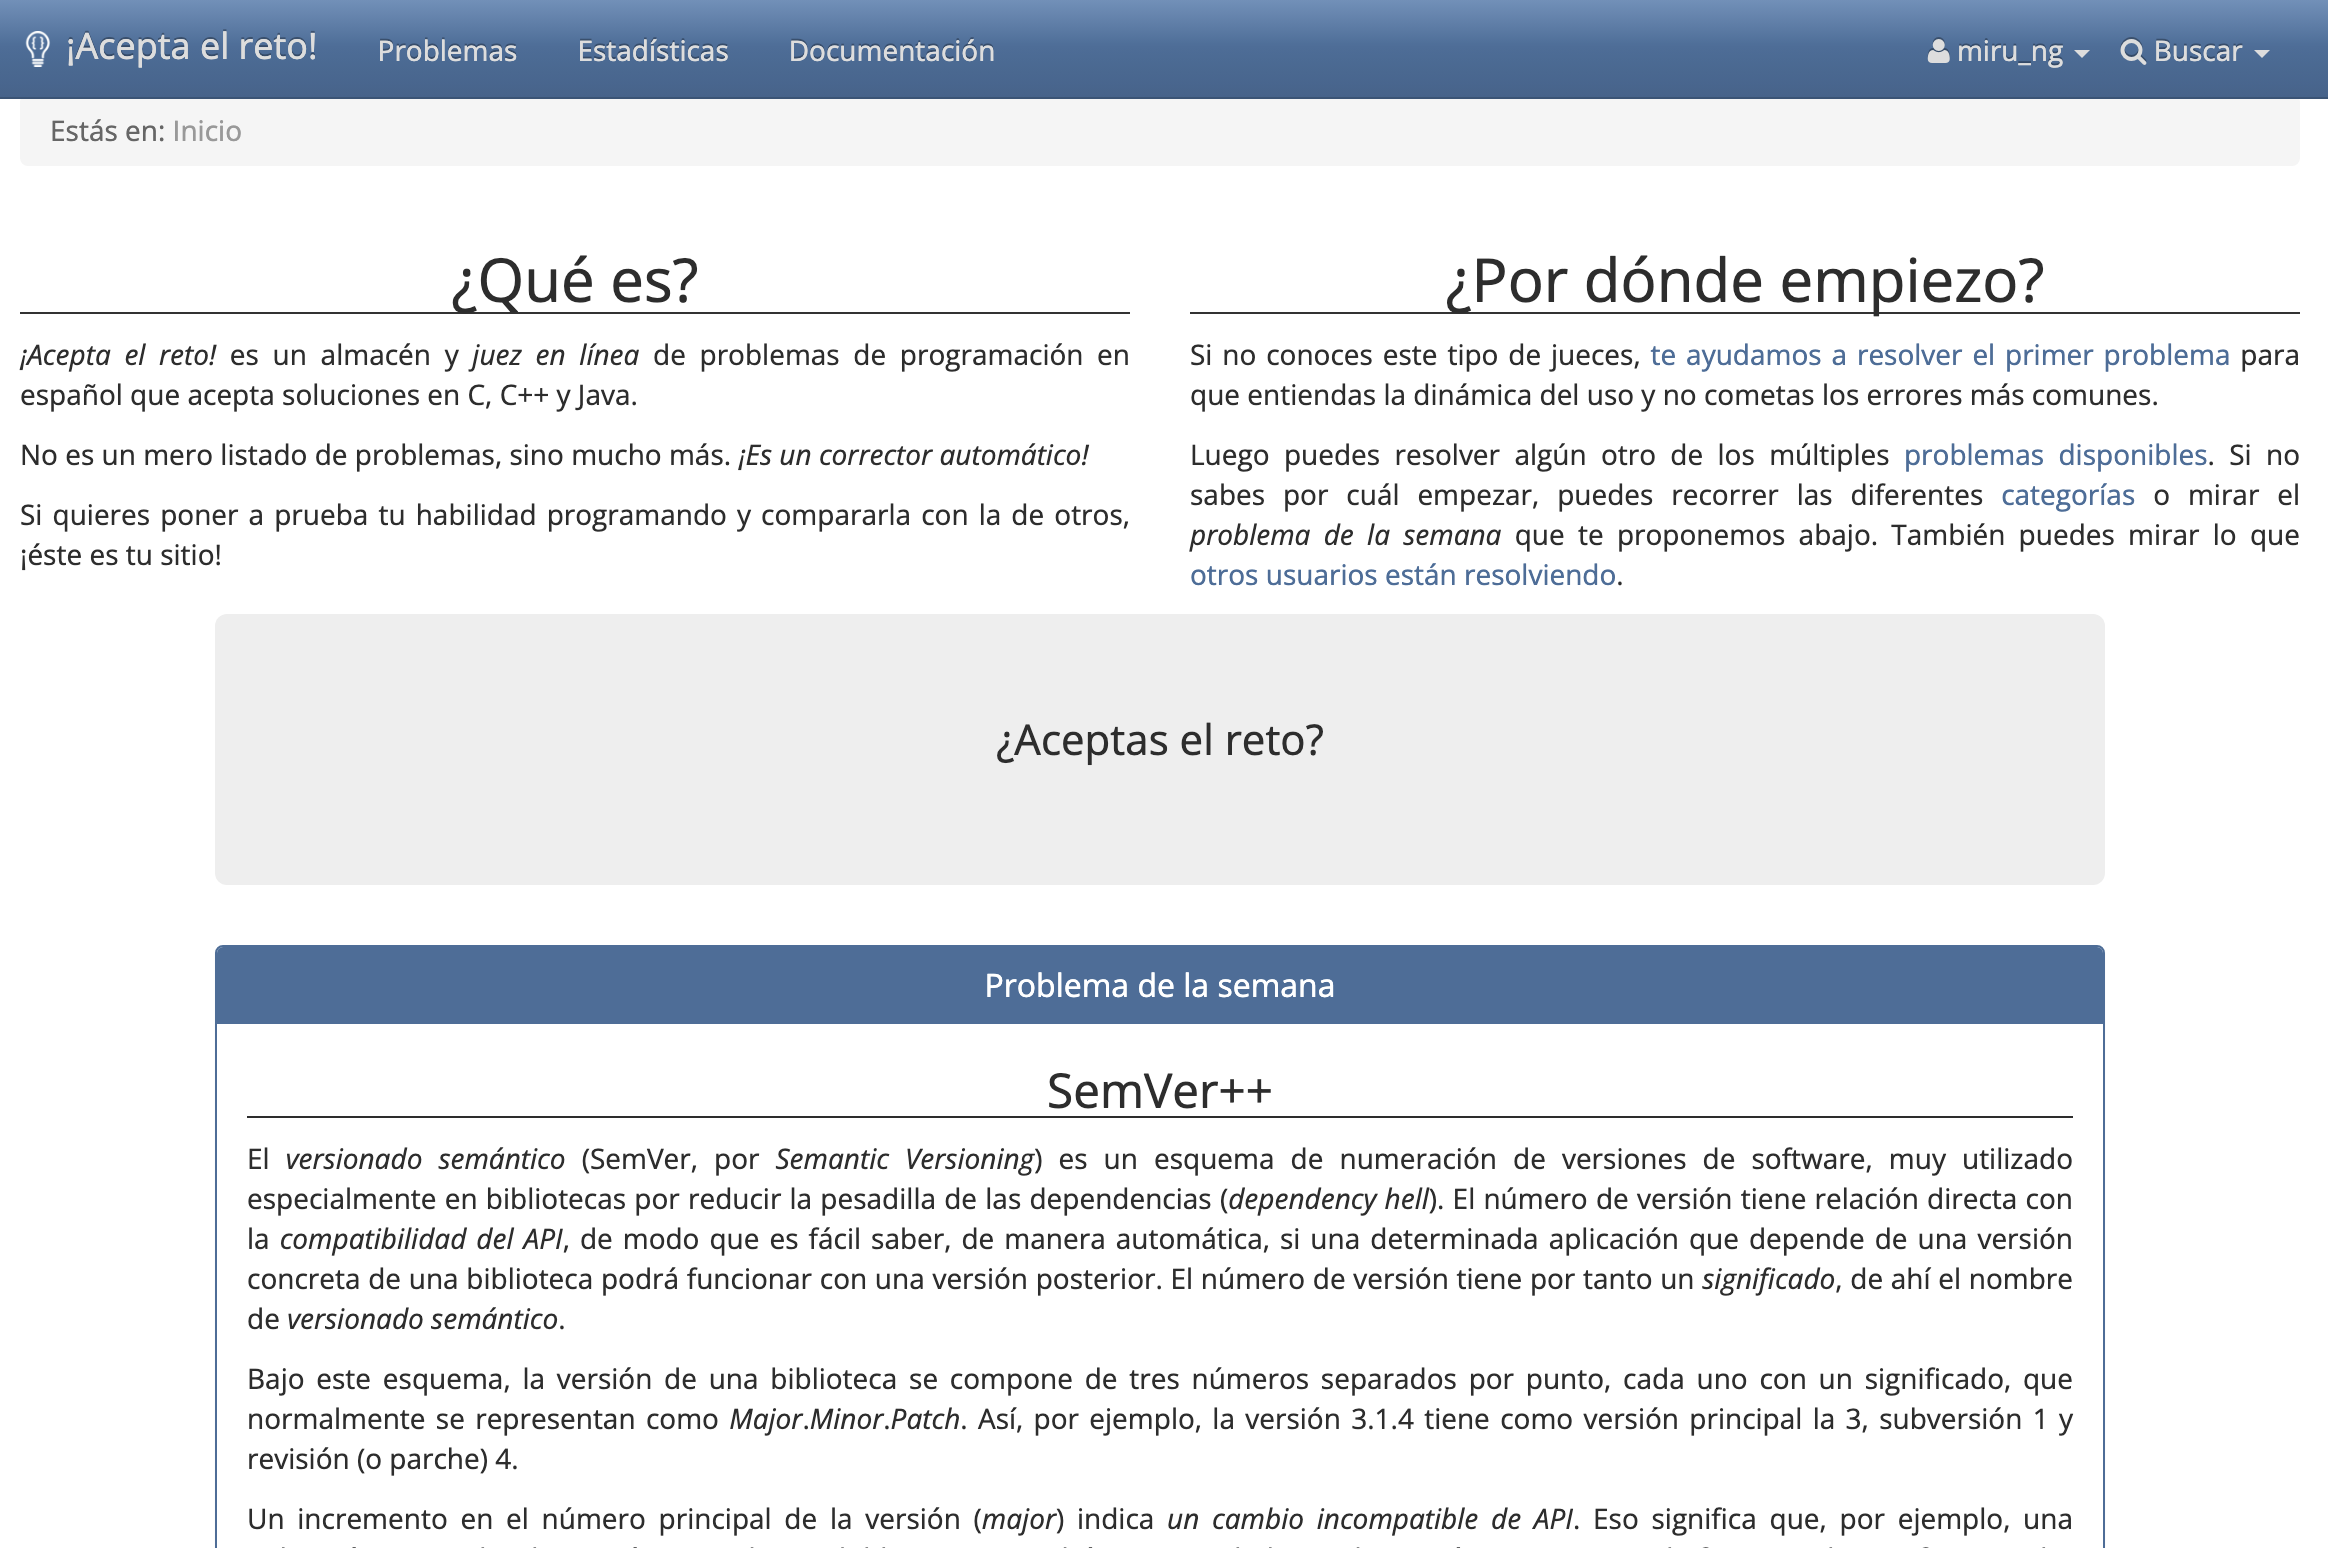
\includegraphics[width = 0.6\textwidth]{Imagenes/Estado del arte/Inicio_AER.png}
	\caption{Inicio Acepta El Reto}
	\label{fig:initAER}
\end{figure}

\textbf{PUNTOS FUERTES:}
\begin{itemize}
    \item \textbf{Gran variedad de problemas:} organizados por categorías, lo que facilita la búsqueda con una interfaz clara y fácil de usar.
    
    \item \textbf{Dentro de cada problema cabe destacar:}
    \begin{itemize}
        \item \textbf{Enunciado en distintos formatos:} directamente en la web, en PDF y en pantalla completa.
        \item \textbf{Apartado de envío intuitivo:} con posibilidad de seleccionar un lenguaje en concreto, añadir un comentario y distintas opciones para subir código (archivo adjunto o editor de código).
        \item \textbf{Estadísticas de las entregas:} lenguaje y veredictos.
        \item \textbf{Historial de envíos.}
    \end{itemize}
    
    \item \textbf{Perfil de usuario muy completo:} además de la información personal, incluye gráficos sobre los lenguajes usados, veredictos y una lista de los problemas enviados a modo de resumen.
\end{itemize}

\textbf{PUNTOS DÉBILES:}
\begin{itemize}
    \item \textbf{Confusión en la navegación:} En la tabla de categorías, casi todas las entradas funcionan como enlaces. Aunque dirigen al mismo destino, esto genera duda e incertidumbre en el usuario.
    
    \item \textbf{Navegación tediosa:} A pesar de que la división por categorías es útil, el proceso de navegar entre ellas exclusivamente a través de tablas resulta lento y poco fluido.
    
    \item \textbf{Estadísticas generales limitadas:} El sistema no ofrece una segmentación por categorías ni datos analíticos relevantes; se limita a mostrar los envíos más recientes de forma global.
    
    \item \textbf{Retroalimentación de errores:} Cuando el código falla, la información proporcionada por la plataforma es poco clara o insuficiente para depurar el error eficientemente.
\end{itemize}


\section{PythonTutor}
Un referente clave para este trabajo es https://pythontutor.com/, cuya principal aportación es la capacidad de generar diagramas automáticos que representan el estado de la memoria durante la ejecución. 

Esta herramienta permite visualizar de forma explícita las estructuras de datos y las relaciones entre ellas mediante punteros y referencias. En el contexto de este TFG, se toma como inspiración el modelo de abstracción visual de Python Tutor para facilitar que el usuario no solo lea el código, sino que comprenda la disposición lógica de las estructuras en la memoria, algo fundamental para evitar errores de lógica.


\begin{figure}[H]
	\centering
	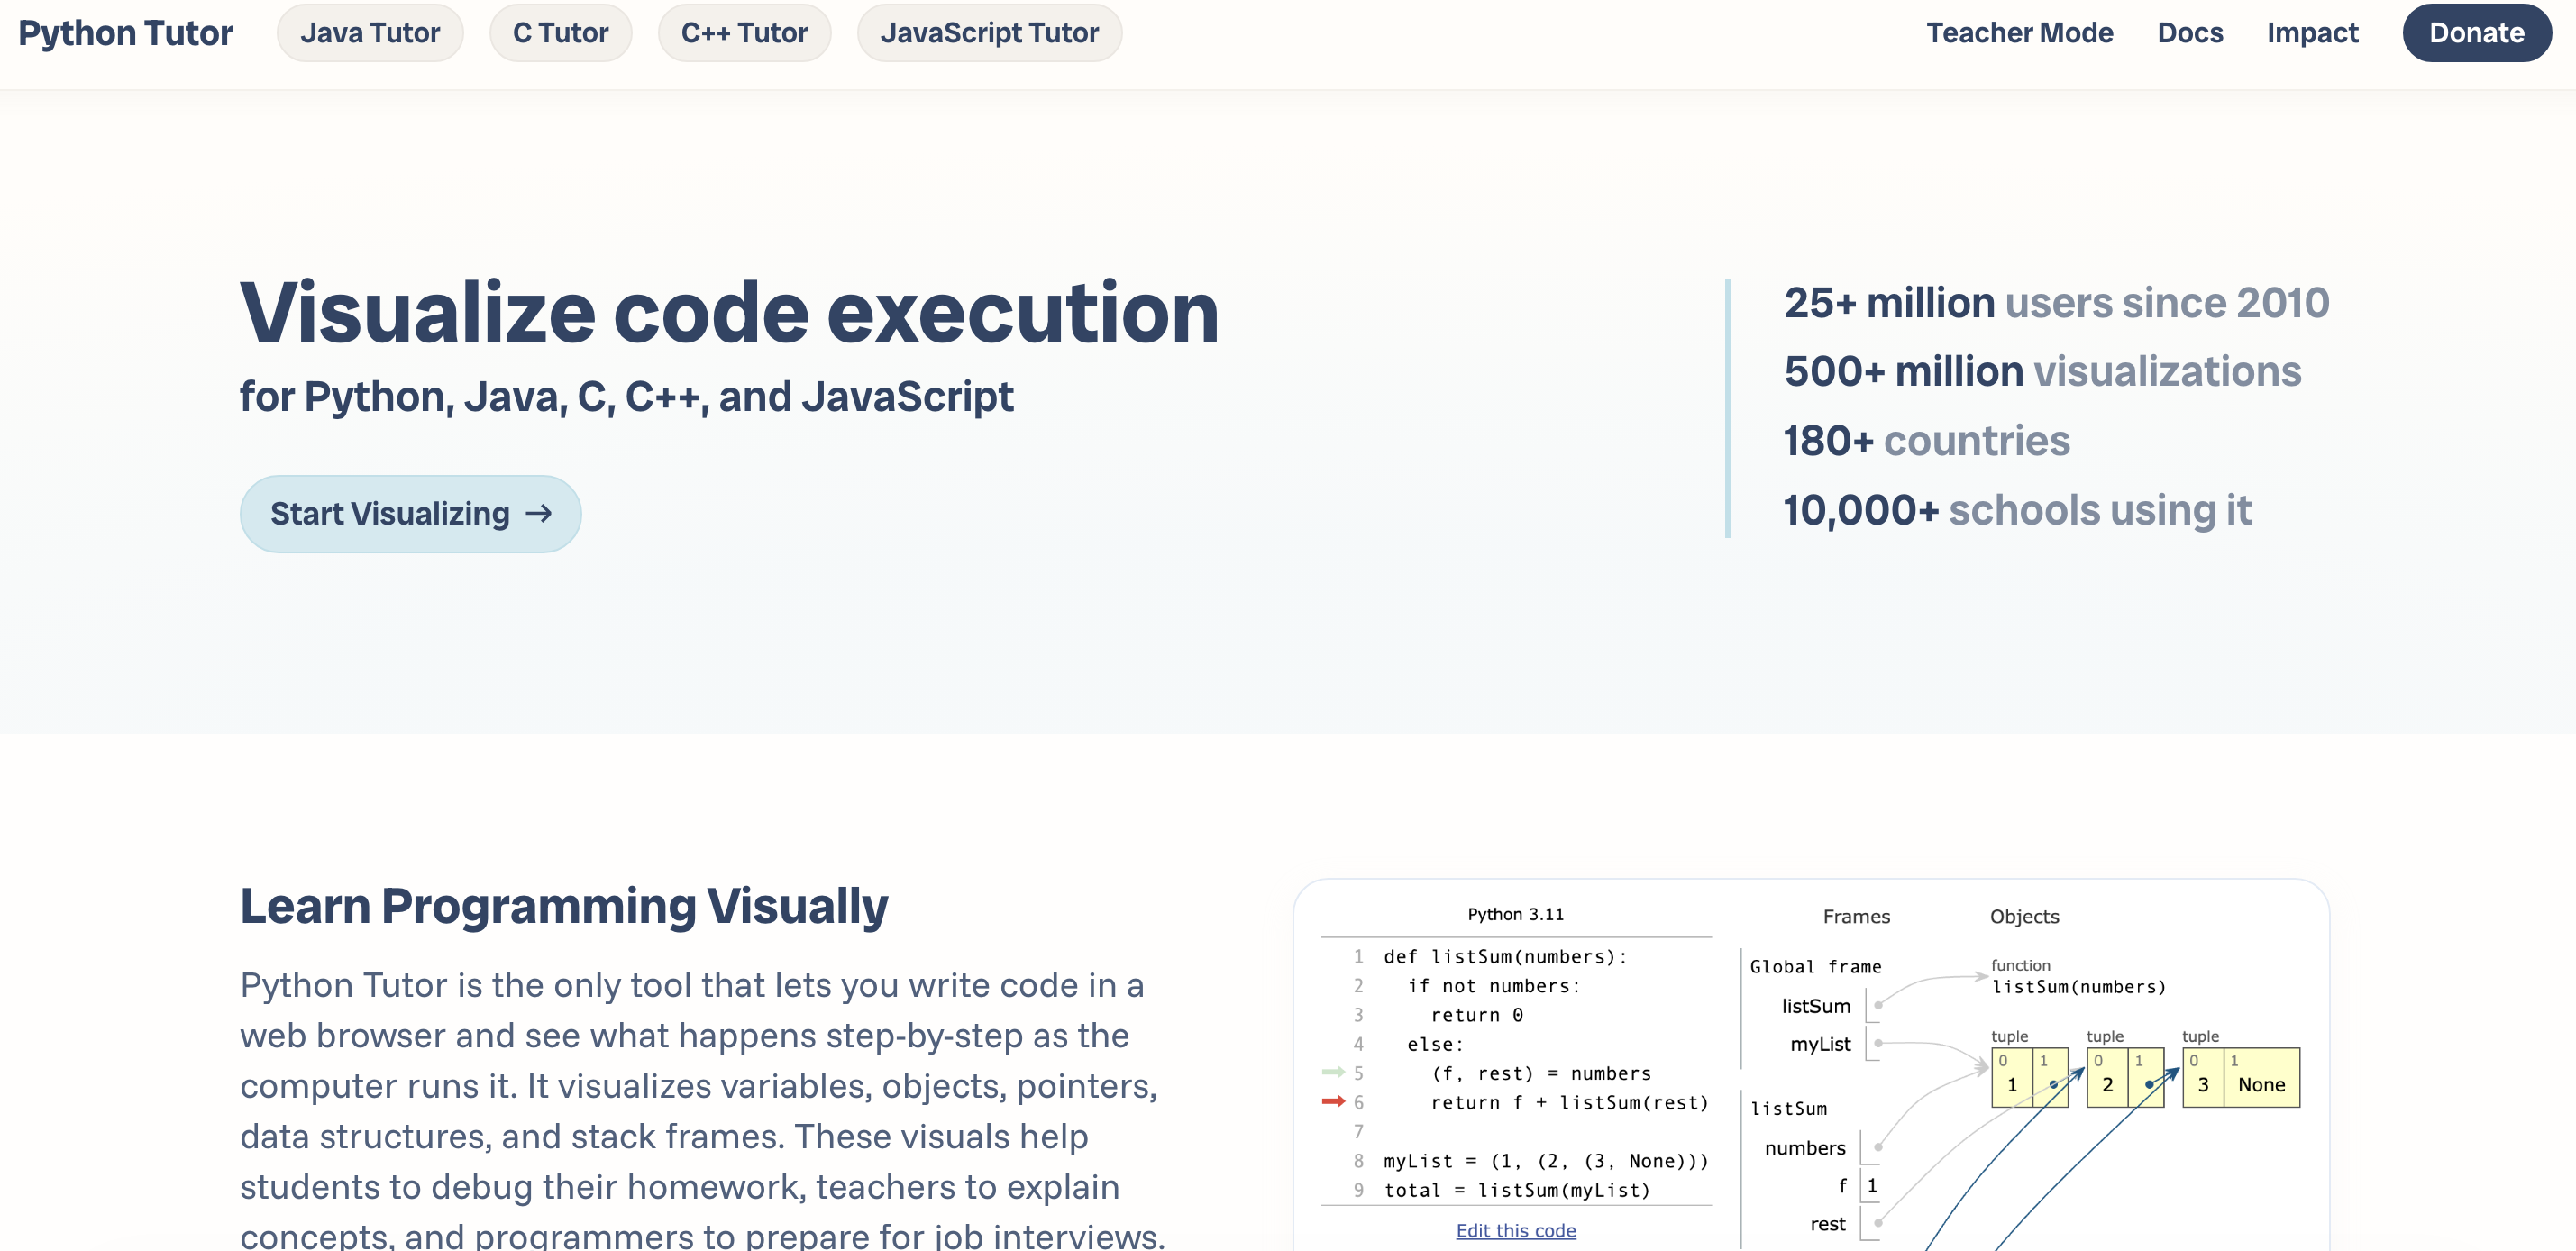
\includegraphics[width = 0.6\textwidth]{Imagenes/Estado del arte/Inicio_PT.png}
	\caption{Inicio Python Tutor}
	\label{fig:initPT}
\end{figure}

\textbf{PUNTOS FUERTES:}
\begin{itemize}
    \item \textbf{Abstracción de la memoria:} separa visualmente dónde viven las variables locales (stack) y dónde se almacenan los objetos complejos como listas o diccionarios (heap).

    \item \textbf{Depuración:} Se puede debuggear hacia adelante o retroceder en el tiempo. Esto permite ver exactamente en qué paso se "rompe" su lógica sin tener que reiniciar toda la ejecución.
    
    \item \textbf{Visualización de punteros:} convierte las referencias de memoria en flechas físicas.
    
    \item \textbf{Lenguaje:} variedad de lenguajes.
\end{itemize}

\textbf{PUNTOS DÉBILES:}
\begin{itemize}
    \item \textbf{Escalabilidad visual:} cuando el código tiene estructuras muy grandes, los diagramas se vuelven difíciles de manejar ya que hay mucho ruido visual. 

    \item \textbf{Explicaciones:} Enseña qué está pasando pero no por qué hay un error o qué significa esa estructura.
    
    \item \textbf{Interfaz anticuada:} solo permite escritura de código, no subir archivos. Además los diagramas no se pueden reorganizar manualmente para mejorar la claridad.
\end{itemize}

\textcolor{red}{FALTA: insertar capturas de todo}
